\documentclass[10pt, conference]{IEEEtran}
\usepackage[english]{babel}
\usepackage[usenames]{color}
\usepackage{colortbl}
\usepackage{comment}
\usepackage{graphicx}
\graphicspath{ {./images/} }
\usepackage{epsfig}
\usepackage{array, colortbl}
\usepackage{listings}
\usepackage{epstopdf}
\usepackage{multirow}
\usepackage{rotating}
\usepackage{subfig}
\usepackage{float}
\usepackage[obeyspaces,hyphens,spaces]{url}
\usepackage{balance}
\usepackage{fancybox}
\usepackage{scalefnt}
\usepackage[normalem]{ulem}
\pagenumbering{arabic}
\pagestyle{empty}
\clubpenalty = 10000
\widowpenalty = 10000
\displaywidowpenalty = 10000
\usepackage{cleveref}
\usepackage{csquotes}
\makeatletter
\renewcommand{\paragraph}[1]{\noindent\textsf{#1}.}

\title{What automated Devops tools can help better understand clients needs 
  throughout the Devops cycle?}
\author{Billy Bouchard, Nicolas Legros    \\
    \emph{billy.bouchard@polymtl.ca, nicolas.legros@polymtl.ca}}

\begin{document}
\maketitle

\begin{abstract}
Understanding clients' needs and getting their feedback has always been 
a critical part of a software's success. However, the techniques and strategies
used in the industry are less than optimal. For instance, 
research shows that up to half of all the features in products are never used~\cite{olsson-helena-15}.\\
The goal of this paper is to aid development teams to improve their process 
in acquiring clients' feedback to better guide their decisions in future development
cycles by providing an analysis on the different tools and strategies used 
in the industry and their characteristics.
\end{abstract}

\section{Problem Statement \& Link with Course}
\label{sec:statement}

Since every piece of software exists to serve a client, wether internal or external,
it's critical that the client's needs stays in the mind of its developers.
However, once the software goes live, updates are always necessary to patch 
some small bugs and add interesting features.
It can be challenging to evaluate what features would be the best or even 
which ones that were succesful.
Moreover, developers sometimes work on features for a long time before 
validating their relevance to their client. It's important to keep the client 
at the center of decisions for new or existing features.
Testing new features or confirming feature success 
by getting customers' feedback can require the creation of focus groups, 
surveys or other more complex systems.
Using devops to create, receive and analyse customer feedback in a timely 
fashion would therefore help development teams in building a successful software.
Indeed, automating the collection of customer feedback and automating the analysis of 
a software's metrics could substantially help development teams to be successful.

\section{Research Questions \& Motivation}
\label{sec:research-idea}

Knowing that the focus of this research will be on the automation of different techniques,
it should come to no suprise that the first part of the research will be to 
find what can actually be automated in the feedback collection process.
\begin{displayquote}
  RQ1. \emph{What feedback techniques can be automatically operated throughout 
  the Devops cycle?}.
\end{displayquote} 
Once there is a sufficient amount of information found on these strategies, we will 
focus on the different metrics leading to RQ2:
\begin{displayquote}
  RQ2. \emph{What feedback metrics can be automatically gathered and processed 
  through logs or other Devops tools and metrics?}.
\end{displayquote} 
Once the compendium of both the techniques and the metrics is found, we 
will be able to focus on their individual usages to see how they are currently 
used in the industry which lead to RQ3:
\begin{displayquote}
  RQ3. \emph{How often are these techniques and metrics implemented in Devops projects?}.
\end{displayquote} 

All these considered, we should be able to better explain what techniques 
seem to be both easier to implement and that yield the best results. 


\section{Data Set \& Analyses}
\label{sec:backgr-relat-work}
% TODO 
Phasellus laoreet ipsum non nunc sodales molestie. Aliquam rutrum urna ante, 
at dictum odio dictum in. Quisque sit amet lorem non mi adipiscing aliquam. 
Suspendisse potenti. Aenean congue a risus vel posuere. Vestibulum tempor 
commodo ipsum vitae congue. Nunc vestibulum volutpat sapien quis tincidunt. 
Vestibulum vitae ullamcorper eros. Integer luctus quam risus~\cite{humble10}. 
Suspendisse scelerisque nulla nulla, sed ullamcorper enim faucibus sed. 
Curabitur bibendum ipsum quis justo tincidunt, et pulvinar enim ullamcorper. 
Pellentesque et tempor turpis. Pellentesque vel nisi metus. Proin laoreet 
vehicula vestibulum. Vivamus iaculis urna velit, et pharetra risus scelerisque quis~\cite{baysal11}.

\section{Two Related Papers}
\label{sec:two-related-papers}

This research should be interesting due to the fact that there is not much research 
on the subject.
However, a ton of corporate articles (e.g. Devops and development lifecycle in 
Google's Cloud Architecture Center) exist and explain some core concepts. 
One of the most interesting papers for this research is written by Google
It explains common metrics that Google uses throughout their devops cycle~\cite{DORA}. 
It goes into the details to explain the importance of both speed and 
regularity when it comes to customer feedback. They present five key metrics to  
implement a good customer feedback cycle and process.
\begin{enumerate}
  \item \emph{Acquisition}: The percentage of users that come to your site who 
    create an account.
  \item \emph{Activation}: The percentage of acquired users that activate their 
    account and use the service.
  \item \emph{Retention}: The percentage of activated users that return to the service.
  \item \emph{Referral}: The percentage of retained users who refer other users to the service.
  \item \emph{Revenue}: The percentage of referring users who actually pay money for the service.
\end{enumerate}
This corporate article is one of the numerous that explain well how to scale 
devops pratices to include customers into the process.\\


Another really interesting article is one from A. Fabijan et al on customer 
feedback and data collection techniques in software R\&D~\cite{fabijan-olsson-15}. 
This article goes in depth to find all the different techniques and metrics 
that the authors could find to qualify and quantitfy customer feedback. 
It gives an incredibly thorough start point to see what techniques and metrics 
this study should analyse and rank.
It explains both the stages at which the techniques must be built, but also the 
limitation each strategy faces.
Therefore, it will be easy to focus on the techniques that can be included in 
a devops cycle as both automated or semi-automated approaches.

\section{Time Planning of Project}
\label{sec:schedule}

The complete paper should be done by December 22 and the poster by November 28. 
It was decided to do a backward analysis to get the most amount of time for 
each parts of the project.
The last month of the project will be allocated to write the report once the 
poster is completed.
Therefore, the research should be completed by November 25 to keep a weekend 
as a buffer. As the metrics evaluation needs to be done once the techniques evaluation is 
completed, the metrics evaluation will start the week before (i.e. November 19).
It would be reasonable to allocate about two weeks to collect all the required 
information on the metrics, which would bring to starting the metrics analysis 
on November 5. 
This means that the techniques analysis will need to be completed by then.
It gives us a total of four weeks to complete the techniques analysis. The 
completed timeline can be seen at figure \ref{fig:timline}.

\begin{figure}[h]
  \caption{Projected timeline for the project}
  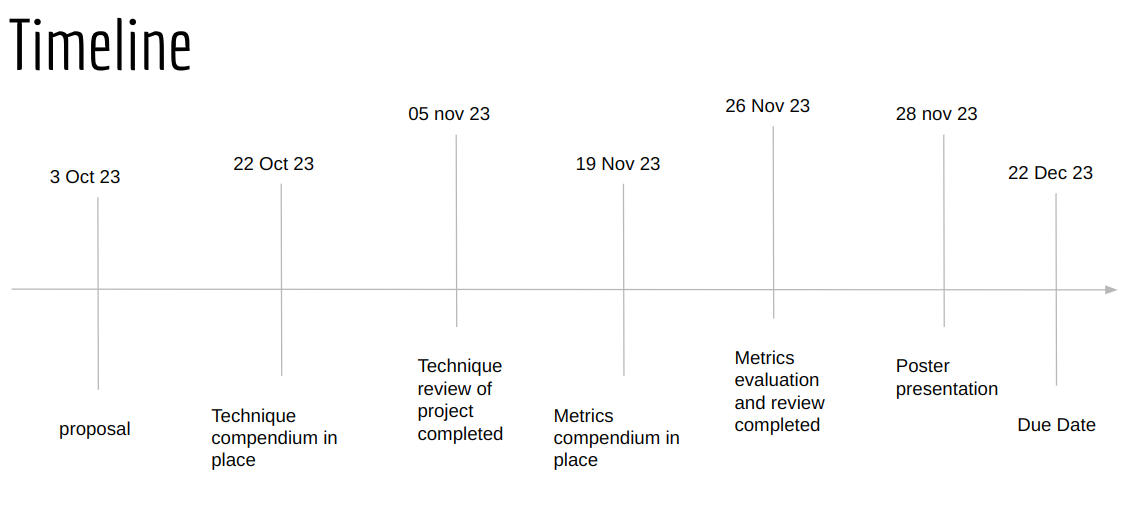
\includegraphics[width=0.5\textwidth]{timeline}
  \label{fig:timline}
\end{figure}

\balance
\bibliographystyle{IEEEtran}
\bibliography{proposal.bib}
\end{document}
